\chapter{Ondes et Particules, Fonction d'onde}

\begin{tcolorbox}
  \begin{itemize}

      \item Onde de de Broglie
        \begin{itemize}

            \item La relation de Einstein-Planck et la relation de de Broglie 
            \item Estimation de l’ordre de grandeur de la longueur de de Broglie pour une particule microscopique ou macroscopique
        \end{itemize}

      \item Fonction d’onde
  \begin{itemize}

        \item Fonction d’onde (amplitude de probabilité), la relation avec la densité de probabilité
        \item Condition de normalisation de la fonction d’onde
        \item Phase additive de la fonction d’onde
        \item Produit scalaire par la notation de Dirac, d ́efinition d’orthogonalité
        \item Statistique : valeur moyenne, incertitude de la position
        \item Exemple : Gaussienne, état localisé, onde de de Broglie (méthode de normalisation)

    \end{itemize}      


  \end{itemize}
\end{tcolorbox}

\section{Introduction}

\subsection{Pourquoi Faire}
Phénomènes expérimentaux imconpréhensible dans le cadre de la physique classique.
        \begin{itemize}
            \item Rayonnement du corp noir, Effet photo électrique : Énergie de rayonnement n'est pas continue, et l'énergie de photon :
                \[
                E = hf = \hbar \omega
                \]
            \item Stabilité d'atom + spectre atomique : Niveau d'énergie atomique discrètes et transition entre deux niveaux $\Delta E$ :
                \[
                \Delta E = hf
                \]
            \item Capacité thermique du solide (cristal) 
        \end{itemize}
\subsection{Phénomène d'interférence}
\textbf{Interférence de Young} : 2 fentes + 1 sonde (détecteur)
\begin{Prop}{Balles (particule)}{}
                \begin{figure}[H] %h:当前位置, t:顶部, b:底部, p:浮动页
                    \centering
                    \includegraphics[width=0.8\textwidth]{./assets/Interférence de Young - Balles.png}
                    \caption{Interférence de Young - Balles}
                    \label{fig:Interfe-rence-de-Young-Balles}
                \end{figure}

                Probabilité totale = sum de probabilité : Interférence de probabilité.
                \[
                    P_{12} = P_1 + P_2
                \]
\end{Prop}

\begin{Prop}{Onde d'eau (onde)}{}
                \begin{figure}[H] %h:当前位置, t:顶部, b:底部, p:浮动页
                    \centering
                    \includegraphics[width=0.8\textwidth]{./assets/Interférence de Young - Onde d'eau.png}
                    \caption{Interférence de Young - Onde d'eau}
                    \label{fig:Interfe-rence-de-Young-Onde-d-eau}
                \end{figure}
                
                Interférence d'amplitude complexe, mais pas l'intensité.
                \[
                    \underline{h_{12}} = \underline{h_1} + \underline{h_2},\; I_{12} \ne I_1 + I_2
                \]
\end{Prop}

\begin{Prop}{Électrons (objet microscopique)}{}
                \begin{figure}[H] %h:当前位置, t:顶部, b:底部, p:浮动页
                    \centering
                    \includegraphics[width=0.8\textwidth]{./assets/Interférence de Young - Électrons.png}
                    \caption{Interférence de Young - Électrons}
                    \label{fig:Interfe-rence-de-Young-E-lectrons}
                \end{figure}
                
                \begin{itemize}
                    \item Frange d'interférence d'électron et l'onde d'eau sont similaires, cela nous inspire de penser que \textit{les objets microscopiques interfèrent comme une onde classique}.
                        \begin{center}
                        Électrons $\iff$ Ondes,\; Amplitude de probabilité$\iff$ Amplitude complexe 
                        \end{center}
                    \item \begin{claim}[colbacktitle=red!75!black]{Fonction d'onde}{}
                Les électrons sont décrit par \textit{une amplitude de probabilité}. Nous l'appelons \textbf{la fonction d'onde}, notant $\psi$, qui est un nombre complex.
                \end{claim}
                    \item Pour une onde classique, intensité = $|\text{amplitude complexe}|^{2}$, et en même temps, pour les électrons, probabilité = $|\text{amplitude de probabilité}|^{2}$.
                        \[
                        P_1 = |\psi_1|^2,\; P_2 = |\psi_2|^2,\; P_{12} = |\psi_1 + \psi_2|^2
                        \]
                    \item Nous conclusons que, pour les électrons, la fonction d'onde s'interferent.
                \end{itemize}
\end{Prop}

\subsection{Électrons : Particule ou onde ?}

\begin{Prop}{Dualité onde-corpuscule}{}
        \begin{itemize}
            \item Les électrons \textit{se propagent} et \textit{interfèrent} comme une onde classique
            \item Les électrons sont \textit{affichés sur écran} comme des particules classiques.
        \end{itemize}

        Conclusion : Ni \textbf{onde classique}, ni \textbf{particule classique}
\end{Prop}

\begin{Theorem}{Relation de Einstein-Planck}{}
        \[
          \boxed{E = \hbar \omega, \; \overrightarrow{p}  = \hbar \overrightarrow{k} \quad (E = pc)}
        \]
\end{Theorem}

\begin{Theorem}{Relation de de Broglie}{}
        \begin{itemize}
            \item Généralisation de photon à tous objets
            \item $\lambda$ propriété ondulatoire,  $p$ propriété particulaire
                 \[
                   \boxed{ \lambda = \frac{h}{p} }
                \]
        \end{itemize}
\end{Theorem}

Application de la relation de de Broglie : \textbf{SEM (Scanning electron microscope)}

\begin{question}{Relation de de Broglie}{}
Mais pourquoi les balles interfèrent pas ? 

\textbf{Réponse :} 

Dans l'exprérience interférence de Young, l'interfrange vaut $\lambda D/a$. Rappelons que la longueur d'onde de de Broglie :
    \[
    \lambda = \frac{h}{p} \text{ avec } p = mv
    \]
\begin{itemize}
    
    \item Pour un électron, $m \approx 10^{-30} \mathrm{kg} $, $v \approx 10^{6} \mathrm{m}/ \mathrm{s}$, $\lambda \approx 10^{-9} \mathrm{m}$, observable.
    \item Pour un balle, $m \approx 10^{-2} \mathrm{kg}$, $v \approx 500 \mathrm{m} / \mathrm{s}$, donc $\lambda \approx 10^{-34} \mathrm{m}$, non-observable.
\end{itemize}

\end{question}

\newpage
\section{Fonction d'onde, Statistiques}

\subsection{Définitions}

\begin{Definition}[colbacktitle=red!75!black]{Fonction d'onde}{}
Toutes les propriétés mécaniques d'une particule peuvent être déterminées de façon \textit{probabilitste} à partir d'une fonction de la position et du temps \underline{à valeurs complexes}:
\begin{center}
  $\boxed{\psi(M,t)}$ appelée \textbf{fonction d'onde} de la particule.
\end{center}
\end{Definition}




\textbf{Différence fondamentale entre classique et quantique} : 
\begin{itemize}
    \item Système \textbf{classique} : décrit par les grandeurs physiques
        \begin{itemize}
            \item Mécanique classique : $\overrightarrow{r}, \overrightarrow{p}$ 
            \item Thermodynamique : $P,U,S,T,V,\ldots$
            \item Électromagnétisme : $\overrightarrow{E} ,\overrightarrow{B} , \rho, \overrightarrow{j} ,\ldots$
        \end{itemize}
    \item Système \textbf{quantique} : décrit uniquement par la fonction d'onde $\psi(M,t)$
\end{itemize}

\begin{Definition}[colbacktitle=red!75!black]{Densité de probabilité de présence}{}
\begin{itemize}
    \item  \textbf{Amplitude de probabilité} : $\psi(M,t)$
    \item  \textbf{Densité de probabilité de présence} au point $M$ à l'instant $t$: $\boxed{\rho(M,t)}$
\end{itemize}
\end{Definition}

\begin{Prop}{Postulat : Relation entre l'amplitude et densité de probabilité de présence}{}
Relation entre $\psi$ et $\rho$
        \[
        \boxed{
        \rho(M,t) = |\psi(M,t)|^{2} = \psi^{*}(M,t) \psi(M,t)}
        \]
\end{Prop}


\begin{note}{}{}
  $\psi$ est semblable à l'amplitude complexe $\underline{A}$ dans l'optique ondulatoire, et $\rho$ semblable à $I$.
\end{note}
\begin{Prop}{Probabilité de trouver la particule dans un volume élémentaire}{}
\begin{itemize}

    \item Probabilité de trouver la particule dans $\mathrm{d} V_M$ à $t$ :
        \[
          \boxed{\mathrm{d} P_{M,t, \mathrm{d} V_m}  = \rho(M,t) \times \mathrm{d} V_M}
        \]

    \item Probabilité de trouver la particule dans $V$ :
        \[
          \boxed{P_{t,V} = \iiint_V \rho(M,t) \mathrm{d} V_M  = \iiint_V |\psi(M,t)|^2 \mathrm{d}V_M = \iiint_V \psi ^* (M,t) \psi(M,t) \mathrm{d} V_M}
        \]
    \item Cas unidimensionnel
      \[
        \mathrm{d}P_{x,t, \mathrm{d}x} = \rho(x, t) \times \mathrm{d}x, \; P _{t,L} = \int _ L \rho(x,t) \mathrm{d}x = \int_L |\psi(x,t)|^2 \mathrm{d}x
      \]

\end{itemize}
\end{Prop}

\begin{Prop}{Dimension de la fonction d'onde}{}
\begin{itemize}

    \item Dimension 3D : $\mathrm{dim} (\rho) = \mathrm{L} ^{-3}$, donc $\mathrm{dim} (\psi) = \mathrm{L} ^{-3 / 2}$. 

\end{itemize}
\end{Prop}
\begin{myproof}{}{}
$P$ pas de dimension, et $\dim V_M = L ^{3}$
\end{myproof}


\subsection{Condition de normalisation} % (fold)
\label{sub:Condition de normalisation}

% subsection Condition de normalisation (end)
\begin{Definition}[colbacktitle=red!75!black]{Condition de normalisation}{}
On peut toujours trouver l'électron qu'on cherche dans tout l'espace, donc, la fonction d'onde doit respecter la \textbf{condition de normalisation} : 

  \begin{itemize}
\item Cas général : \[
          \boxed{\iiint_{\text{tout l'espace}} \rho(M,t)\mathrm{d} V_M = \iiint_{\text{tout l'espace}} |\psi(M,t)|^{2}\mathrm{d} V_M = \iiint_{\text{tout l'espace}} \psi ^* (M,t) \psi(M,t)\mathrm{d} V_M = 1}
        \]
    \item Cas unidimensionnel
        \[
        \int_{-\infty}^{+\infty} |\psi(M,t)|^{2}\mathrm{d} x = \displaystyle\int_{- \infty}^{ + \infty} \psi_1 ^{*}(x,t) \psi_2(x,t) \mathrm{d}x = 1
        \]

    (On va utiliser la notation de l'intégration du cas unidimensionnel)
  \end{itemize}
\end{Definition}


\begin{Prop}{Espace Hilbertien}{}
$\psi \in \mathcal{L}^{2}$ (Espace Hilbertien, espace vectoriel complexe muni d'un produit scalaire hermitien), le module au carré de la fonction $\psi(x,t)$ doit être sommable
\end{Prop}

\begin{Prop}{}{}
    Densité de probabilité inchangé en multipliant $e^{i\alpha}$ avec $\alpha$  \textit{constant}.
        \[
          \boxed{\psi' = \psi \times \exp(i \alpha) \text{ avec } \alpha = C _{te} \implies |\psi'|^{2} = |\psi|^{2}}
        \]
\end{Prop}


\begin{Definition}[colbacktitle=red!75!black]{Phase de la fonction d'onde}{}
Comme $\alpha$ ne change pas la probabilité de présence, 
\begin{center}
    La phase de la fonction d'onde est définie à une constante additive près : $\alpha$ indépendant de $M$
\end{center}
\end{Definition}


\subsection{Produit scalaire - Notation de Dirac} % (fold)

% subsection  (end)

\begin{Definition}[colbacktitle=red!75!black]{Notation de Dirac - Produit scalaire de fonction d'onde}{}
Produit scalaire (hermitien) s'écrit sous la \textbf{notation de Dirac}
\[
  \boxed{  \langle \psi_1 | \psi_2 \rangle = \int _{- \infty} ^{+ \infty} \psi_1^{*}(M,t) \psi_2(M,t) \mathrm{d} V_M}
\]

Norme d'une fonction d'onde : 
\[
\Vert \psi  \Vert ^{2}  = \langle \psi | \psi \rangle
\]
\end{Definition}

\begin{Prop}{Notation de Dirac}{}
Propriétés :
\begin{itemize}
    \item $\langle \psi_1 | \psi_2 \rangle = \langle \psi_2 | \psi_1 \rangle ^{*}$
    \item $\langle \psi_1 | \lambda \psi_2 \rangle = \lambda \langle \psi_1 | \psi_2 \rangle $ 
    \item $\langle \lambda \psi_1 | \psi_2 \rangle = \lambda^{*} \langle \psi_1 | \psi_2 \rangle $
    \item $\langle \psi_1 | \psi_2 + \psi_3 \rangle = \langle \psi_1 | \psi_2 \rangle + \langle \psi_1 | \psi_3 \rangle$
    \item $\langle \psi_1 + \psi_2 | \psi_3 \rangle = \langle \psi_1 | \psi_3 \rangle + \langle \psi_2 | \psi_3 \rangle$
\end{itemize}
\end{Prop}

\begin{Prop}{Condition de normalisation sous la notation de Dirac}{}
  $$\boxed{\langle \psi | \psi \rangle =1}$$
\end{Prop}
\begin{Definition}[colbacktitle=red!75!black]{Orthogonalité de la fonction d'onde}{}
  Orthogonalité : $\psi_1$ et $\psi_2$ sont \textbf{orthogonaux} si $$\boxed{\langle \psi_1 | \psi_2 \rangle =0}$$
\end{Definition}




\begin{question}{}{}
Si $\psi$ est normalisé, écrire la relation vérifiée de $\alpha_1$ et $\alpha_2$, la condition de normalisation de $\psi = \alpha _1\psi_1 + \alpha _2 \psi_2$ su $\psi_1$ et $\psi_2$ sont normalisées et orthogonaux.
\end{question}

\begin{myproof}
\begin{align*}
    \langle \psi | \psi \rangle = 1 &\implies \int( \alpha _1\psi_1 + \alpha _2\psi_2)^{*}( \alpha _1 \psi_1 + \alpha _2\psi_2 )\mathrm{d} V \\ 
                                    &\implies |\alpha_1|^2 \int \psi_1 ^* \psi_1 + \alpha_1 ^* \alpha_2 \int \psi_1 ^* \psi_2 + \alpha_2 ^* \alpha_1 \int \psi_2 ^* \psi_1 + | \alpha_2| ^2 \int \psi_2 ^* \psi_2 = 1 \\
                                    &\implies |\alpha_1|^2 \langle \psi_1 | \psi_1 \rangle + \alpha_1 ^* \alpha_2 \langle \psi_1 ^* \psi_2 \rangle + \alpha_2 ^* \alpha_1 \langle \psi_2 | \psi_1 \rangle + | \alpha_2 | ^2 \langle \psi_2 | \psi_1 \rangle = 1 \\
                                    &\implies |\alpha_1|^2 + |\alpha_2| ^2 = 1
\end{align*}
\end{myproof}

\subsection{Prédiction statistiques}

\begin{Definition}[colbacktitle=red!75!black]{Position moyenne}{}
    \begin{itemize}
      \item 1D : \[
          \boxed{\langle x \rangle = \int_{-\infty}^{+\infty} x \rho(x,t) \mathrm{d}x = \displaystyle\int_{-\infty}^{+\infty} \varphi ^{*} (x,t) x \varphi(x, t) \mathrm{d}x}
    \]
  \item 3D : \[
      \langle \overrightarrow{OM} \rangle = \iiint _{\text{Tout l'espace}} \psi ^* (M,t) \;\overrightarrow{OM} \;\psi(M,t) \;\mathrm{d}V _M
  \]
    
    \end{itemize}
\end{Definition}

\begin{Definition}[colbacktitle=red!75!black]{Largeur de distribution}{}
Dans le cas unidimensionnel, la \textbf{largeur de distribution}, notée $\Delta x$ est définie par :
\[
  \boxed{ \Delta x = \sqrt{ \langle x ^2 \rangle - \langle x \rangle ^2}} 
\]

La largeur $\Delta x$ caractérise l'\underline{étalement de la fonction d'onde} : Une faible largeur signifie que la particule est bien localisé.

$\Delta x$ peut être considéré comme une incertitude fondamentale. 
\end{Definition}

\begin{Prop}{Grandeurs dépendant de la position}{}
La \textbf{valeur moyenne} et la \textbf{largeur statistique de la distribution} de $f(M,t)$ sont données par :
\[
  \boxed{\langle f(M,t) \rangle = \iiint \psi ^*(M,t) f(M,t) \psi(M,t) \mathrm{d}V_M, \quad \Delta f = \sqrt{ \langle f ^2(M,t) \rangle - \langle f(M,t) \rangle ^2}} 
\]

\end{Prop}


\subsection{Distribution Gaussienne} % (fold)
\label{sub:Distribution Gaussienne}

% subsection Distribution Gaussienne (end)
\begin{Example}{Distribution Gaussienne 1D}{}
\begin{itemize}
    \item Distribution de Gauss 1D : \[
        \boxed{   f(x) = \frac{1}{\sigma \sqrt{2\pi}} \exp \left(-\frac{(x-\mu)^2}{2 \sigma ^2}\right)} 
    \]
    vérifiant $\langle x \rangle = \mu$, $\langle x ^2 \rangle = \sigma ^2 + \mu ^2$, $\Delta x = \sigma$
  \item Fonction d'onde de forme gaussienne : Comme \underline{$|\psi_L(x)|^2$ est une distribution de Gauss 1D}, on remplace $\sigma$ par $L$ et $\mu$ par $x_0$, \[
    \boxed{\psi_L(x) = \frac{1}{(2 \pi L ^2)^{\color{red}{1 / 4}}} \exp\left( - \frac{(x-x_0) ^2}{{\color{red}{4}} L ^2}\right)}  
  \]
  vérifiant $\langle x \rangle = x_0$ et $\Delta x = L$
\end{itemize}

\begin{figure}[H] %h:当前位置, t:顶部, b:底部, p:浮动页
  \centering
  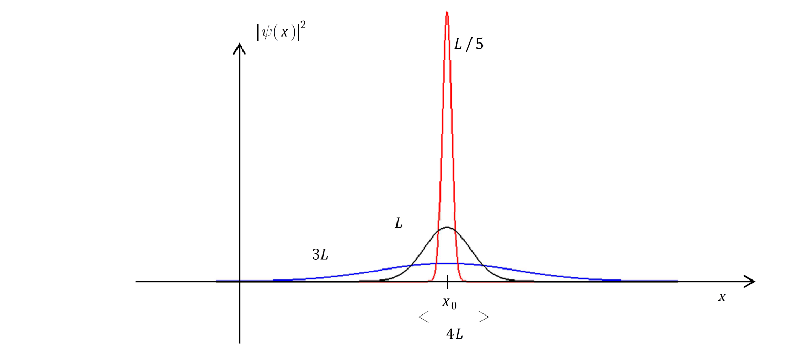
\includegraphics[width=0.8\textwidth]{./assets/Fonction d'onde Gaussienne 1D.png}
  \caption{Fonction d'onde Gaussienne 1D}
  \label{fig:Fonction d'onde Gaussienne 1D}
\end{figure}


\end{Example}

\subsection{Distribution de Dirac} % (fold)
\label{sub:Distribution de Dirac}

% subsection Distribution de Dirac (end)

\begin{Example}{Distribution de Dirac}{}
À partir de l'exemple précédent, lorsque $L \to 0$, toutes les mesures de position donneront la même valeur $x_0$. Donc, 

\begin{Definition}[colbacktitle=red!75!black]{Distribution de Dirac}{}
On définie la \textbf{distribution de Dirac}, la limite d'une suite de fonction $(\psi_L) _{L \in \mathbb{R}}$ : \[
  \boxed{\delta(x-x_0) =  \underset{L \to 0}{\mathrm{lim}} \psi_L ^2(x)}
\]
\end{Definition}

\begin{Prop}{Propriétés de la distribution de Dirac}{}
\begin{itemize}
    \item Normalisé : 
      \[
        \int_{- \infty}^{ + \infty} \delta(x-x_0) \mathrm{d} x = 1
      \]
    \item Échantillonnage : Une particule qui se trouve dans l'état $\psi _{L \to 0} (x)$ a une position parfaitement déterminée.
      \[
        \boxed{\int _{- \infty}^{+ \infty}f(x) \delta(x-x_0) \mathrm{d}x = f(x_0)}
      \] 
    \item {\color{red} Relation importante}
      \[
        \boxed{        \delta(x) = \frac{1}{2 \pi} \int _{- \infty}^{+ \infty}\exp{ikx} \mathrm{d}k}
      \] 
    \item Utilisé pour décrire une distribution ponctuelle.

\end{itemize}
\end{Prop}

État de la position défini : $\psi _{x_0} = \delta(x-x_0)$, $\langle x \rangle=x_0$, $\Delta x = 0$ (d'un point de vue physique).
\end{Example}

\subsection{Ondes de de Broglie} % (fold)
\label{sub:Ondes de de Broglie}

% subsection Ondes de de Broglie (end)
Pour une particule libre, la \textbf{Relation de de Broglie} relie $\lambda$ et $p$ et $\overrightarrow{k}$ le vecteur d'onde, et l'énergie à la pulsation : grandeurs ne sont définies que pour une OPPM.
\begin{Definition}[colbacktitle=red!75!black]{Ondes de de Broglie}{}
Les \textbf{ondes de de Broglie} : états de \underline{quantité de mouvement} bien définie :
\[
  \psi _{\overrightarrow{p}} ( M,t) = A \exp [i( \overrightarrow{k}. \overrightarrow{OM} - \omega t)] = \boxed{A \exp \left[ \frac{i}{\hbar}( \overrightarrow{p}. \overrightarrow{OM} - Et)\right]}
\]
avec $\overrightarrow{p} = \hbar \overrightarrow{k}$, $E = \hbar \omega$

\end{Definition}

\begin{Prop}{Normalisation de ondes de de Broglie}{}
\begin{itemize}

    \item Ils ne peuvent pas être normalisées dans tout l'espace :
      \[
        \displaystyle\int_{- \infty}^{+ \infty} | \psi_p(x,t) | ^{2} \mathrm{d} x = \int_{- \infty}^{+ \infty} |A| ^{2} \mathrm{d} x \to \infty
      \]
    \item Méthodes de normalisation (1D) : Dans $x \in [-L _{\max}/2, L _{\max}/2]$, 
    \[
      \boxed{\psi_p(x,t) = \frac{1}{\sqrt{L_{\max}}} \exp \left[ \frac{i}{\hbar}(p x -Et)\right]}
    \]
    \item Méthodes de normalisation (3D) : Dans $x \in V _{\max}$, 
    \[
      \psi_{\overrightarrow{p}}(x,t) = \frac{1}{\sqrt{V_{\max}}} \exp \left[ \frac{i}{\hbar}( \overrightarrow{p}. \overrightarrow{OM} -Et)\right]
    \]

\end{itemize}
\end{Prop}

\begin{Prop}{Probabilité de présence}{}
$\forall M, \;| \psi_p(M,t) | ^{2} = |A| ^{2}$ donc la densité de probabilité de présence est uniforme. Cela implique que la particule peut se trouver n'importe où dans la région considérée, avec la même probabilité.
\end{Prop}



\subsection{Principe de superposition} % (fold)

\begin{Prop}{Énoncé de la principe de superposition}{}
Si $\psi_1(M,t)$ et $\psi_2(M,t)$ deux fonctions d'ondes possibles pour le système considéré, alors : 
\center
$\psi(M,t) = \alpha_1 \psi_1(M,t) + \alpha_b \psi_2(M,t)$ est également une fonction d'onde possible pour le système.
\end{Prop}


% subsection  (end)
